\documentclass{article}
\usepackage[T1]{fontenc}
\usepackage{lmodern}
\usepackage{graphicx}
\usepackage{amsmath,amssymb}
\usepackage[a4paper,margin=2cm]{geometry}
\usepackage[absolute,overlay]{textpos}
\setlength{\TPHorizModule}{1mm}
\setlength{\TPVertModule}{1mm}
\usepackage[indonesian]{babel}
\usepackage{hyperref}
\setlength{\emergencystretch}{2em}
% unit: Halaman 58

\begin{document}

% === Halaman 58 (llm) ===

\section*{Tiga (3) Jenis Algoritma Kriptografi}

\subsection*{1. Algoritma kriptografi simetri (symmetric-key cryptography)}
\begin{itemize}
    \item Kunci enkripsi = kunci dekripsi, harus dijaga privat (rahasia) atau \textit{secret}
    \item Sudah ada sejak ribuan tahun yang hingga tahun 1976
\end{itemize}

\vspace{30mm}

\begin{itemize}
    \item Data Encryption Standard (DES)
    \item Advanced Encryption Standard (AES)
    \item Serpent
    \item Blowfish
    \item Loki
    \item MARS
    \item RC6
    \item Twofish
    \item 3-DES
    \item IDEA
    \item FEAL
    \item RC4
    \item SEAL
    \item Panama
    \item dll
\end{itemize}

% deskripsi: Diagram proses enkripsi dan dekripsi menggunakan kriptografi kunci simetri, menunjukkan input Plainteks P yang dienkripsi dengan Kunci privat K menjadi Cipherteks C, lalu didekripsi kembali dengan Kunci privat K menjadi Plainteks P.
% bbox normalisasi: [0.1600, 0.4500, 0.7600, 0.7100]
\begin{textblock*}{126.00mm}(33.60mm,133.65mm)
\noindent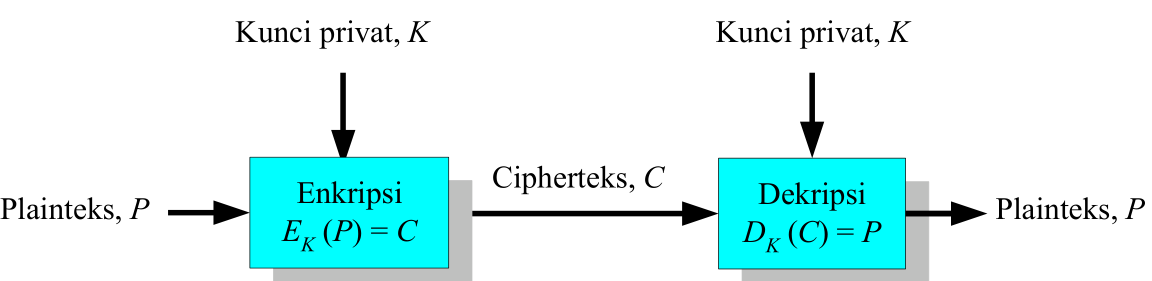
\includegraphics[width=126.00mm,height=77.22mm]{../../images/llm/page_058_img_01.png}%
\end{textblock*}

\end{document}
